\documentclass{article}
\usepackage{amsmath}
\usepackage{amsfonts}
\usepackage{tikz}
\usetikzlibrary{patterns}

\begin{document}
\begin{figure}[htbp]
\begin{center}
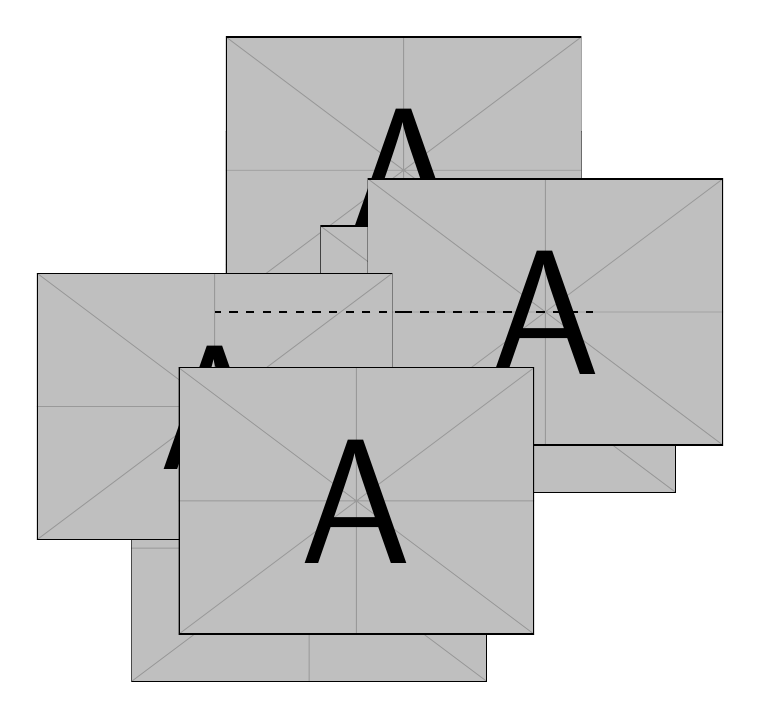
\begin{tikzpicture}[scale=0.6]
\node at (-2,-5) {\includegraphics[scale=0.4]{example-image-a}};
\node at (-2,-2) {\includegraphics[scale=0.4]{example-image-a}};
\node at (0,1) {\includegraphics[scale=0.4]{example-image-a}};
\node at (0,3) {\includegraphics[scale=0.4]{example-image-a}};
\node at (2,-1) {\includegraphics[scale=0.4]{example-image-a}};
\node at (3,0) {\includegraphics[scale=0.4]{example-image-a}};
\node at (-4,-2) {\includegraphics[scale=0.4]{example-image-a}};
\node at (-1,-4) {\includegraphics[scale=0.4]{example-image-a}};
\draw[dashed] (0,0)--(4,0);
\draw[dashed] (0,0)--(-4,0);
\end{tikzpicture}
\end{center}
\caption{}
\label{fig:lamb13}
\end{figure}
\end{document}